\documentclass[12pt]{article}

\usepackage{sbc-template}
\usepackage{graphicx,url}
\usepackage{enumitem}
\usepackage[brazil]{babel} 
%\usepackage[latin1]{inputenc}
\usepackage[utf8x]{inputenc}
\usepackage{multirow}
\usepackage[table]{xcolor}
     
\sloppy

\title{Usando Certificados Digitais OM-BR para proteção de Medidores de Combustível}
% \author{Nome do Autor\inst{1}}
% 
% \address{Endereço Linha 1\\
%   Endereço Linha 2
%   \email{\{email\}@email.do.aut}
% }

\author{
  Wilson S. Melo Jr.\inst{1}, Raphael C. Machado \inst{1}, Bruno Abreu\inst{1},\\ 
  Ruy Ramos\inst{2}, Luiz F. R. C. Carmo\inst{1,3}}
\address{Instituto Nacional de Metrologia, Qualidade e Tecnologia (Inmetro)\\
  Duque de Caxias, RJ -- Brasil
\nextinstitute
  Instituto Nacional de Tecnologia da Informação\\
  Brasília -- Brasil
\nextinstitute
  Universidade Federal do Rio de Janeiro (UFRJ)\\
  Programa de Pós-Graduação em Informática (PPGI) -- Rio de Janeiro, RJ -- Brasil  
\email{\{wsjunior,rcmachado,beabreu,lfrust\}@inmetro.gov.br, ruy@iti.gov.br}
}

\begin{document} 

\maketitle

%\begin{abstract}
%\end{abstract}
     
%\begin{resumo} 
%\end{resumo}

\section{Introdução}
No mundo todo, a metrologia legal tem o desafio de prover à sociedade a confiabilidade de instrumentos de medição usados em diferentes atividades e relações de consumo.
Nos países em desenvolvimento, tal desafio torna-se ainda mais complexo em função do elevado número de fraudes associadas a esses instrumentos.
Somente no Brasil, Rodrigues et al. sugere que o prejuízo causado à sociedade em função de fraudes em medição é superior a XXX.
Essas fraudes geralmente ocorrem quando uma entidade maliciosa tenta adulterar as respostas fornecidas por um instrumento de medição, obtendo assim vantagens indevidas na comercialização de um determinado bem.

Nesse cenário, os medidores de combustível, vulgarmente conhecidos como \emph{bombas de combustível}, são talvez os instrumentos mais visados em termos de fraudes e adulteração de medidas.
A literatura relata problemas relacionados a estes instrumentos em diferentes países, tais como Brasil, México e Nigéria.
A fraude associada à medição de combustível pode ser extremamente lucrativa, e ao mesmo tempo difícil de ser exposta.
Isso motiva especialmente a ação de vendedores de combustível maliciosos, que deliberadamente adulteram o medidor de combustível em uma categoria de fraude conhecida como "bomba baixa".

Por mais que o Inmetro intensifique esforços na fiscalização dos medidores de combustível, tal tarefa é complexa em virtude do elevado número de equipamentos e da capilaridade de distribuição destes pelo país.
Tais características tornam a fiscalização extremamente custosa e mesmo ineficiente contra mecanismos de fraude que podem ser furtivos e facilmente desabilitados pelo atacante na iminência de uma inspeção.

Em face dessas dificuldades, muitos esforços tem sido feitos no sentido de tornar o medidor de combustível um instrumento mais robusto a eventuais ataques.
A ideia consiste em se propor requisitos de segurança e proteção de software que são expressos em Regulamentos Técnicos Metrológicos (RTMs).
Tais requisitos, por sua vez, são verificados pelo Inmetro durante as atividades de aprovação de modelo (type approval), previstas na Metrologia Legal como um importante processo para se garantir a confiabilidade metrológica de um instrumento de medição.
Nesse escopo, e com base em pesquisas desenvolvidas não somente pelo Inmetro, mas também por outros institutos de metrologia em outros países, o Inmetro propôs a inclusão de dois requisitos essenciais para se garantir a integridade, autenticidade e não repúdio de uma medição:

\begin{itemize}
    \item O uso de assinatura digital do registro legalmente relevante do instrumento, no momento mais próximo possível da concretização de uma medição, e;
    \item O uso de certificados digitais padrão ICP-Brasil, que são aqueles em conformidade com a Infraestrutura de Chave Pública oficial do país.
\end{itemize}

Neste artigo, são descritos de forma detalhada como cada um dos requisitos contribui para a proteção das medições realizados por um medidor de combustível.
Inicialmente, apresenta-se uma visão geral do funcionamento de uma bomba de combustível, e como um de seus componentes, o \textit{pulser}, pode ser construído como um elemento seguro que fornece apenas valores de medição devidamente assinados.
Em seguida, discute-se a adoção de certificados digitais específicos para dispositivos de medição, e como os mesmos agregam confiabilidade ao processo de medição como um todo, tornando-se uma ferramenta de apoio às atividades da metrologia legal.

\section{Como funciona uma bomba de combustível}
Um medidor de combustível basicamente bombeia o combustível de um tanque subterrâneo, passando por um transdutor de medição responsável pela medição.
O combustível segue então por um duto ou mangueira, sob o controle de uma válvula solenóide, sendo por fim injetado por meio de um bico no tanque do carro.
O transdutor é tipicamente representado por um eixo mecânico integrado a um pulsador.
O movimento do eixo é convertido em pulsos eletrônicos, de modo que o número de pulsos é proporcional ao volume medido.
Em função disso, o conjunto mecânico que inclui o transdutor é denominado \textit{pulser}.
A Figura \ref{f:transducer} ilustra o funcionamento do \textit{pulser} em um típico modelo de medidor de combustível.

\begin{figure}[ht]
\centering
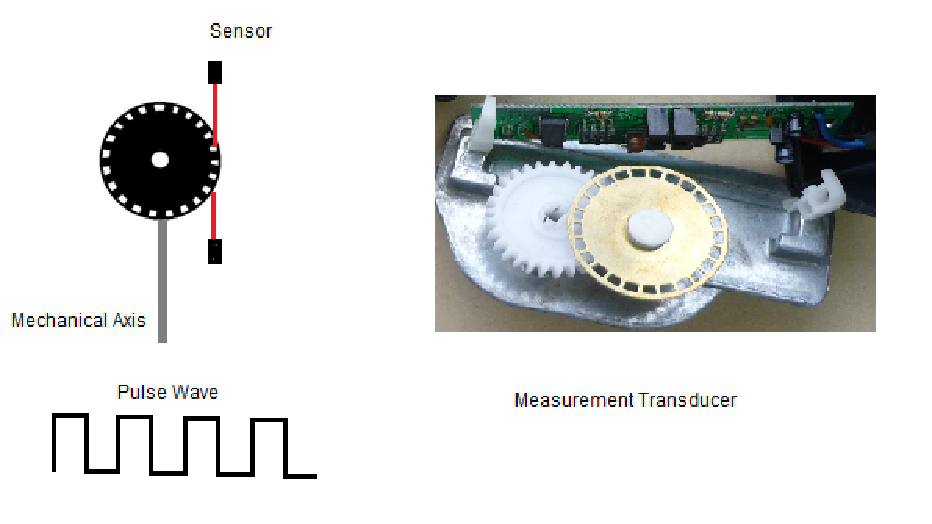
\includegraphics[width=0.9\textwidth]{transducer}
\caption{Princípio de funcionamento de um medidor de combustível}
\label{f:transducer}
\end{figure}



\begin{figure}[ht]
\centering
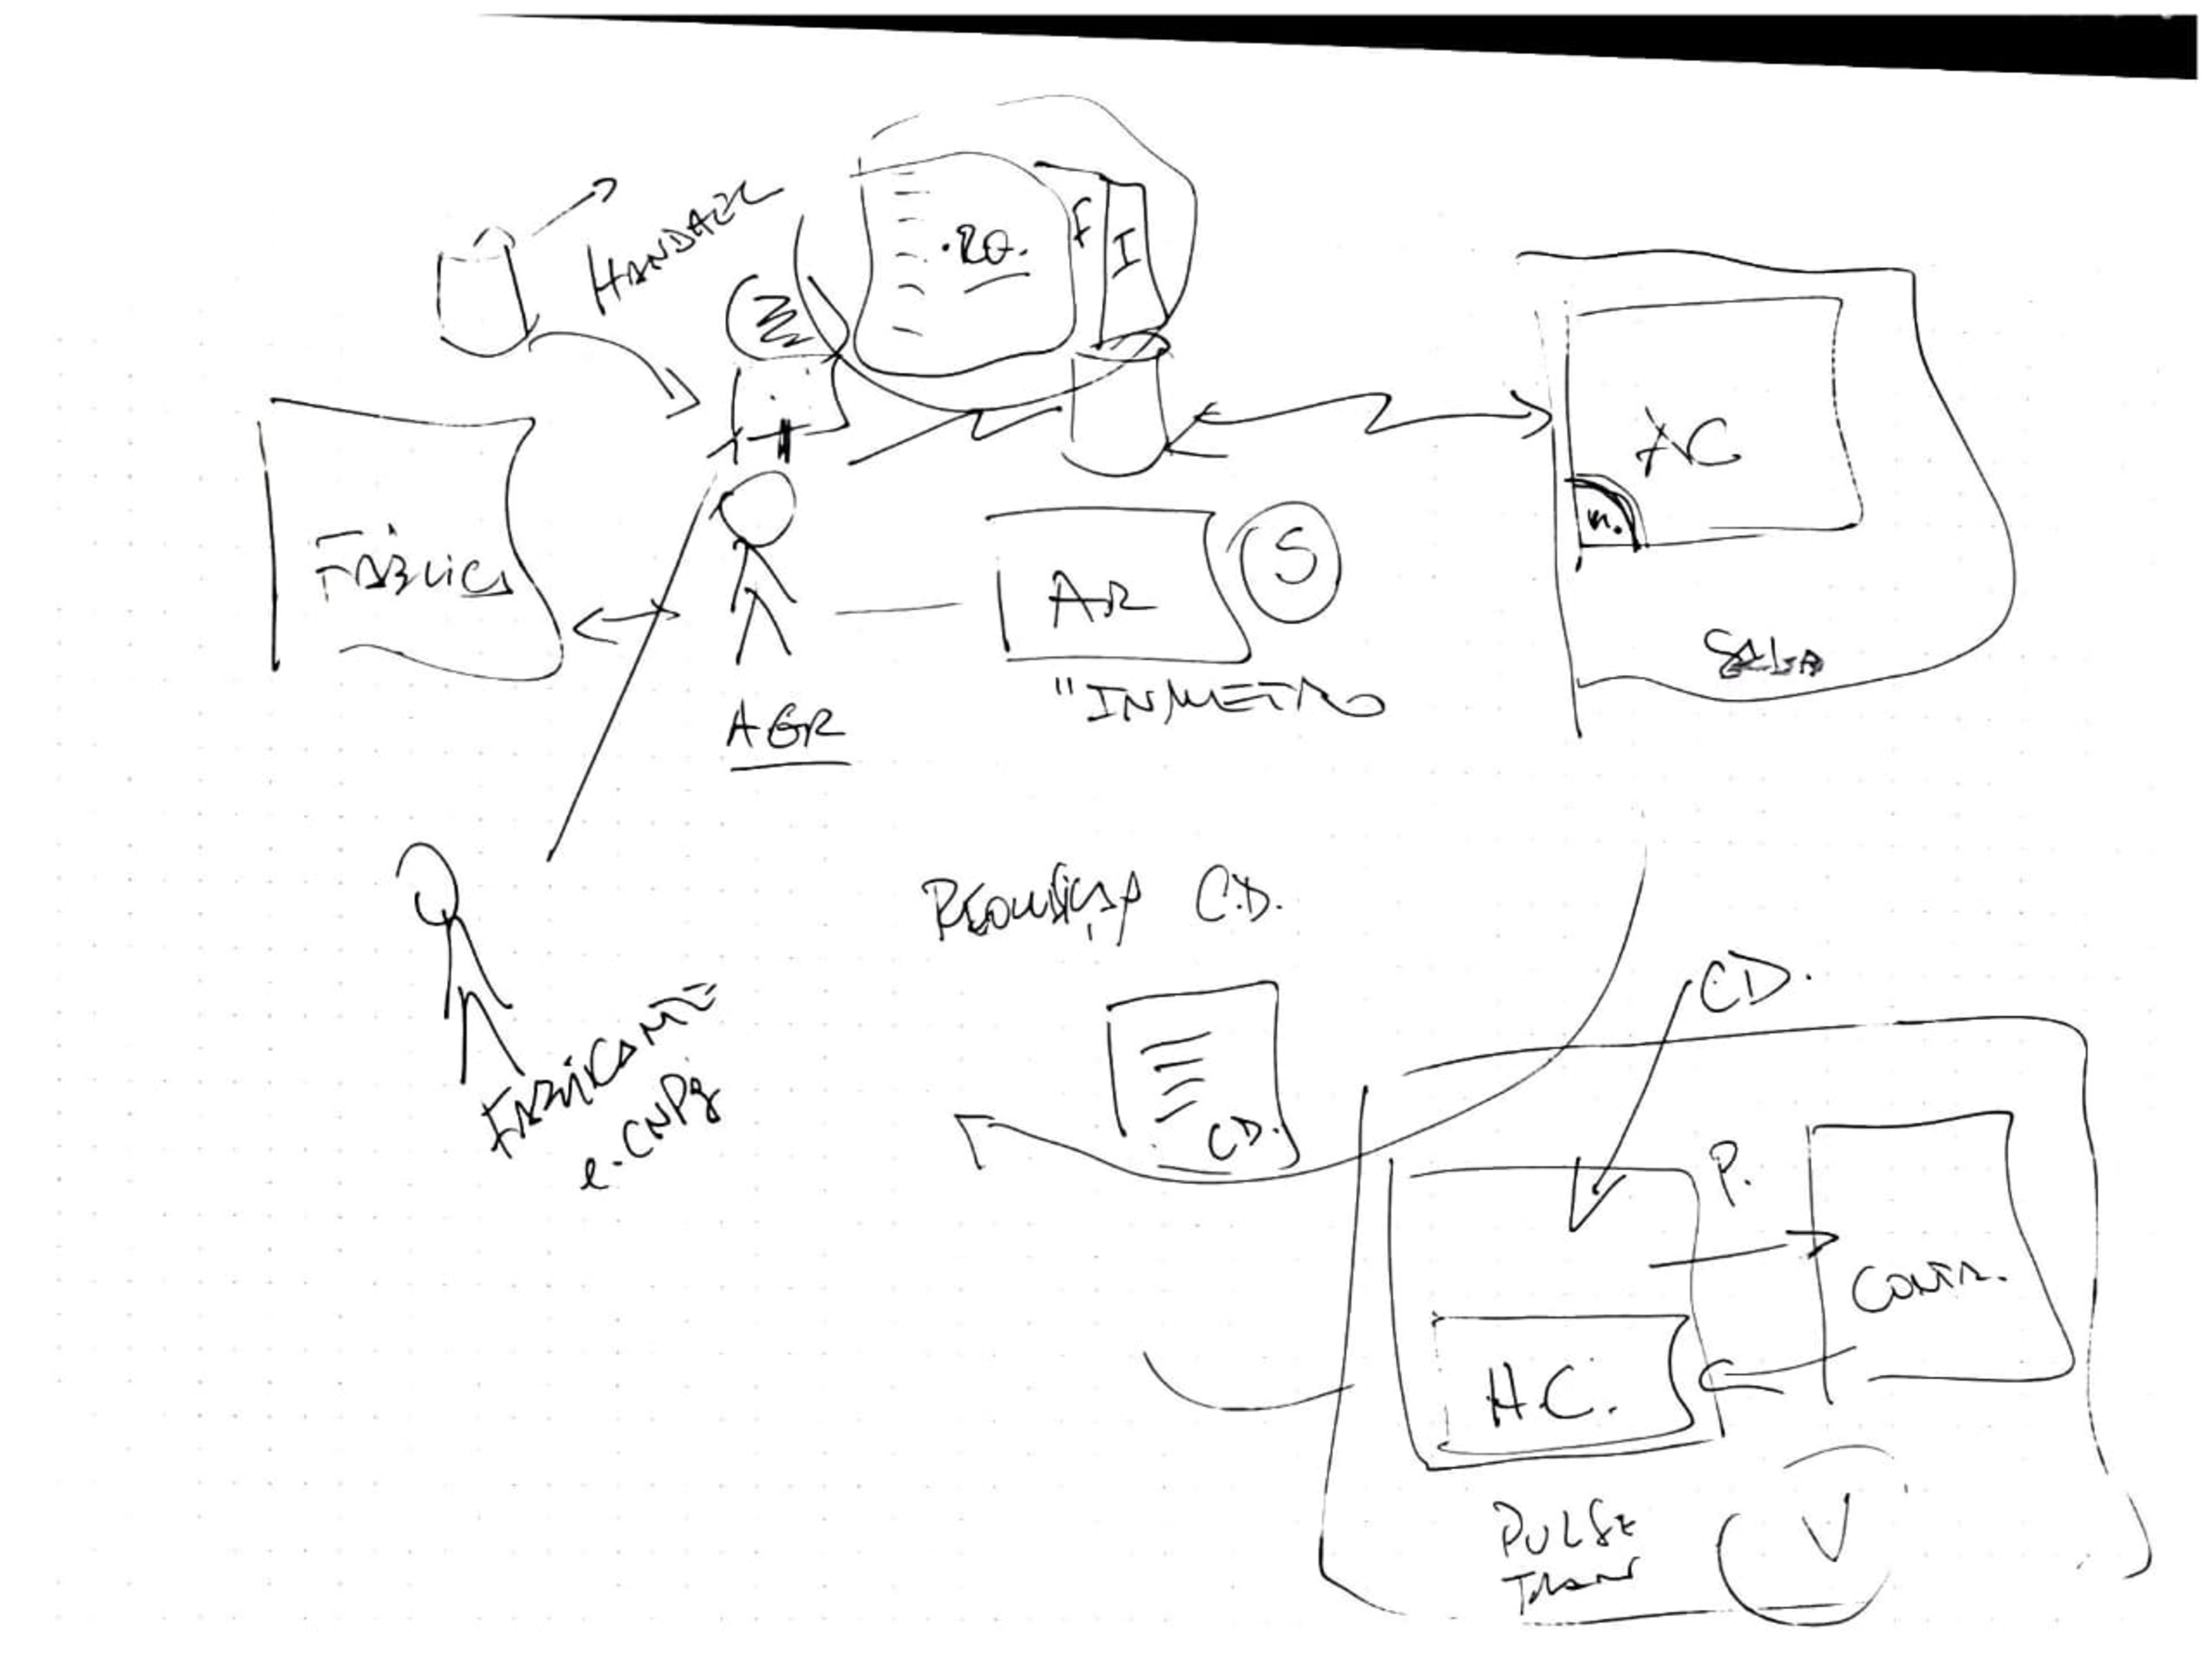
\includegraphics[width=1\textwidth]{ruy.pdf}
\caption{Diagrama descrevendo papéis de AR e AC}
\label{f:ruy}
\end{figure}

%\pagebreak

% Figure and table captions should be centered if less than one line
% (Figure~\ref{fig:exampleFig1}), otherwise justified and indented by 0.8cm on
% both margins, as shown in Figure~\ref{fig:exampleFig2}. The caption font must
% be Helvetica, 10 point, boldface, with 6 points of space before and after each
% caption.
% 
% \begin{figure}[ht]
% \centering
% \includegraphics[width=.5\textwidth]{fig1.jpg}
% \caption{A typical figure}
% \label{fig:exampleFig1}
% \end{figure}
% 
% \begin{figure}[ht]
% \centering
% \includegraphics[width=.3\textwidth]{fig2.jpg}
% \caption{This figure is an example of a figure caption taking more than one
%   line and justified considering margins mentioned in Section~\ref{sec:figs}.}
% \label{fig:exampleFig2}
% \end{figure}
% 
% In tables, try to avoid the use of colored or shaded backgrounds, and avoid
% thick, doubled, or unnecessary framing lines. When reporting empirical data,
% do not use more decimal digits than warranted by their precision and
% reproducibility. Table caption must be placed before the table (see Table 1)
% and the font used must also be Helvetica, 10 point, boldface, with 6 points of
% space before and after each caption.
% 
% \begin{table}[ht]
% \centering
% \caption{Variables to be considered on the evaluation of interaction
%   techniques}
% \label{tab:exTable1}
% \includegraphics[width=.7\textwidth]{table.jpg}
% \end{table}

\bibliographystyle{sbc}
\bibliography{sbc-template}

\end{document}
